\item El siguiente \textbf{modelo E-R} (figura \ref{fig:2ii}) corresponde a una base de datos de una universidad. Luego de unos años de funcionamiento, se han detectado una \textbf{serie de deficiencias en el sistema de mantenimiento de datos} y se quieren realizar las \textbf{siguientes modificaciones}:

\begin{figure}[H]
	\centering
	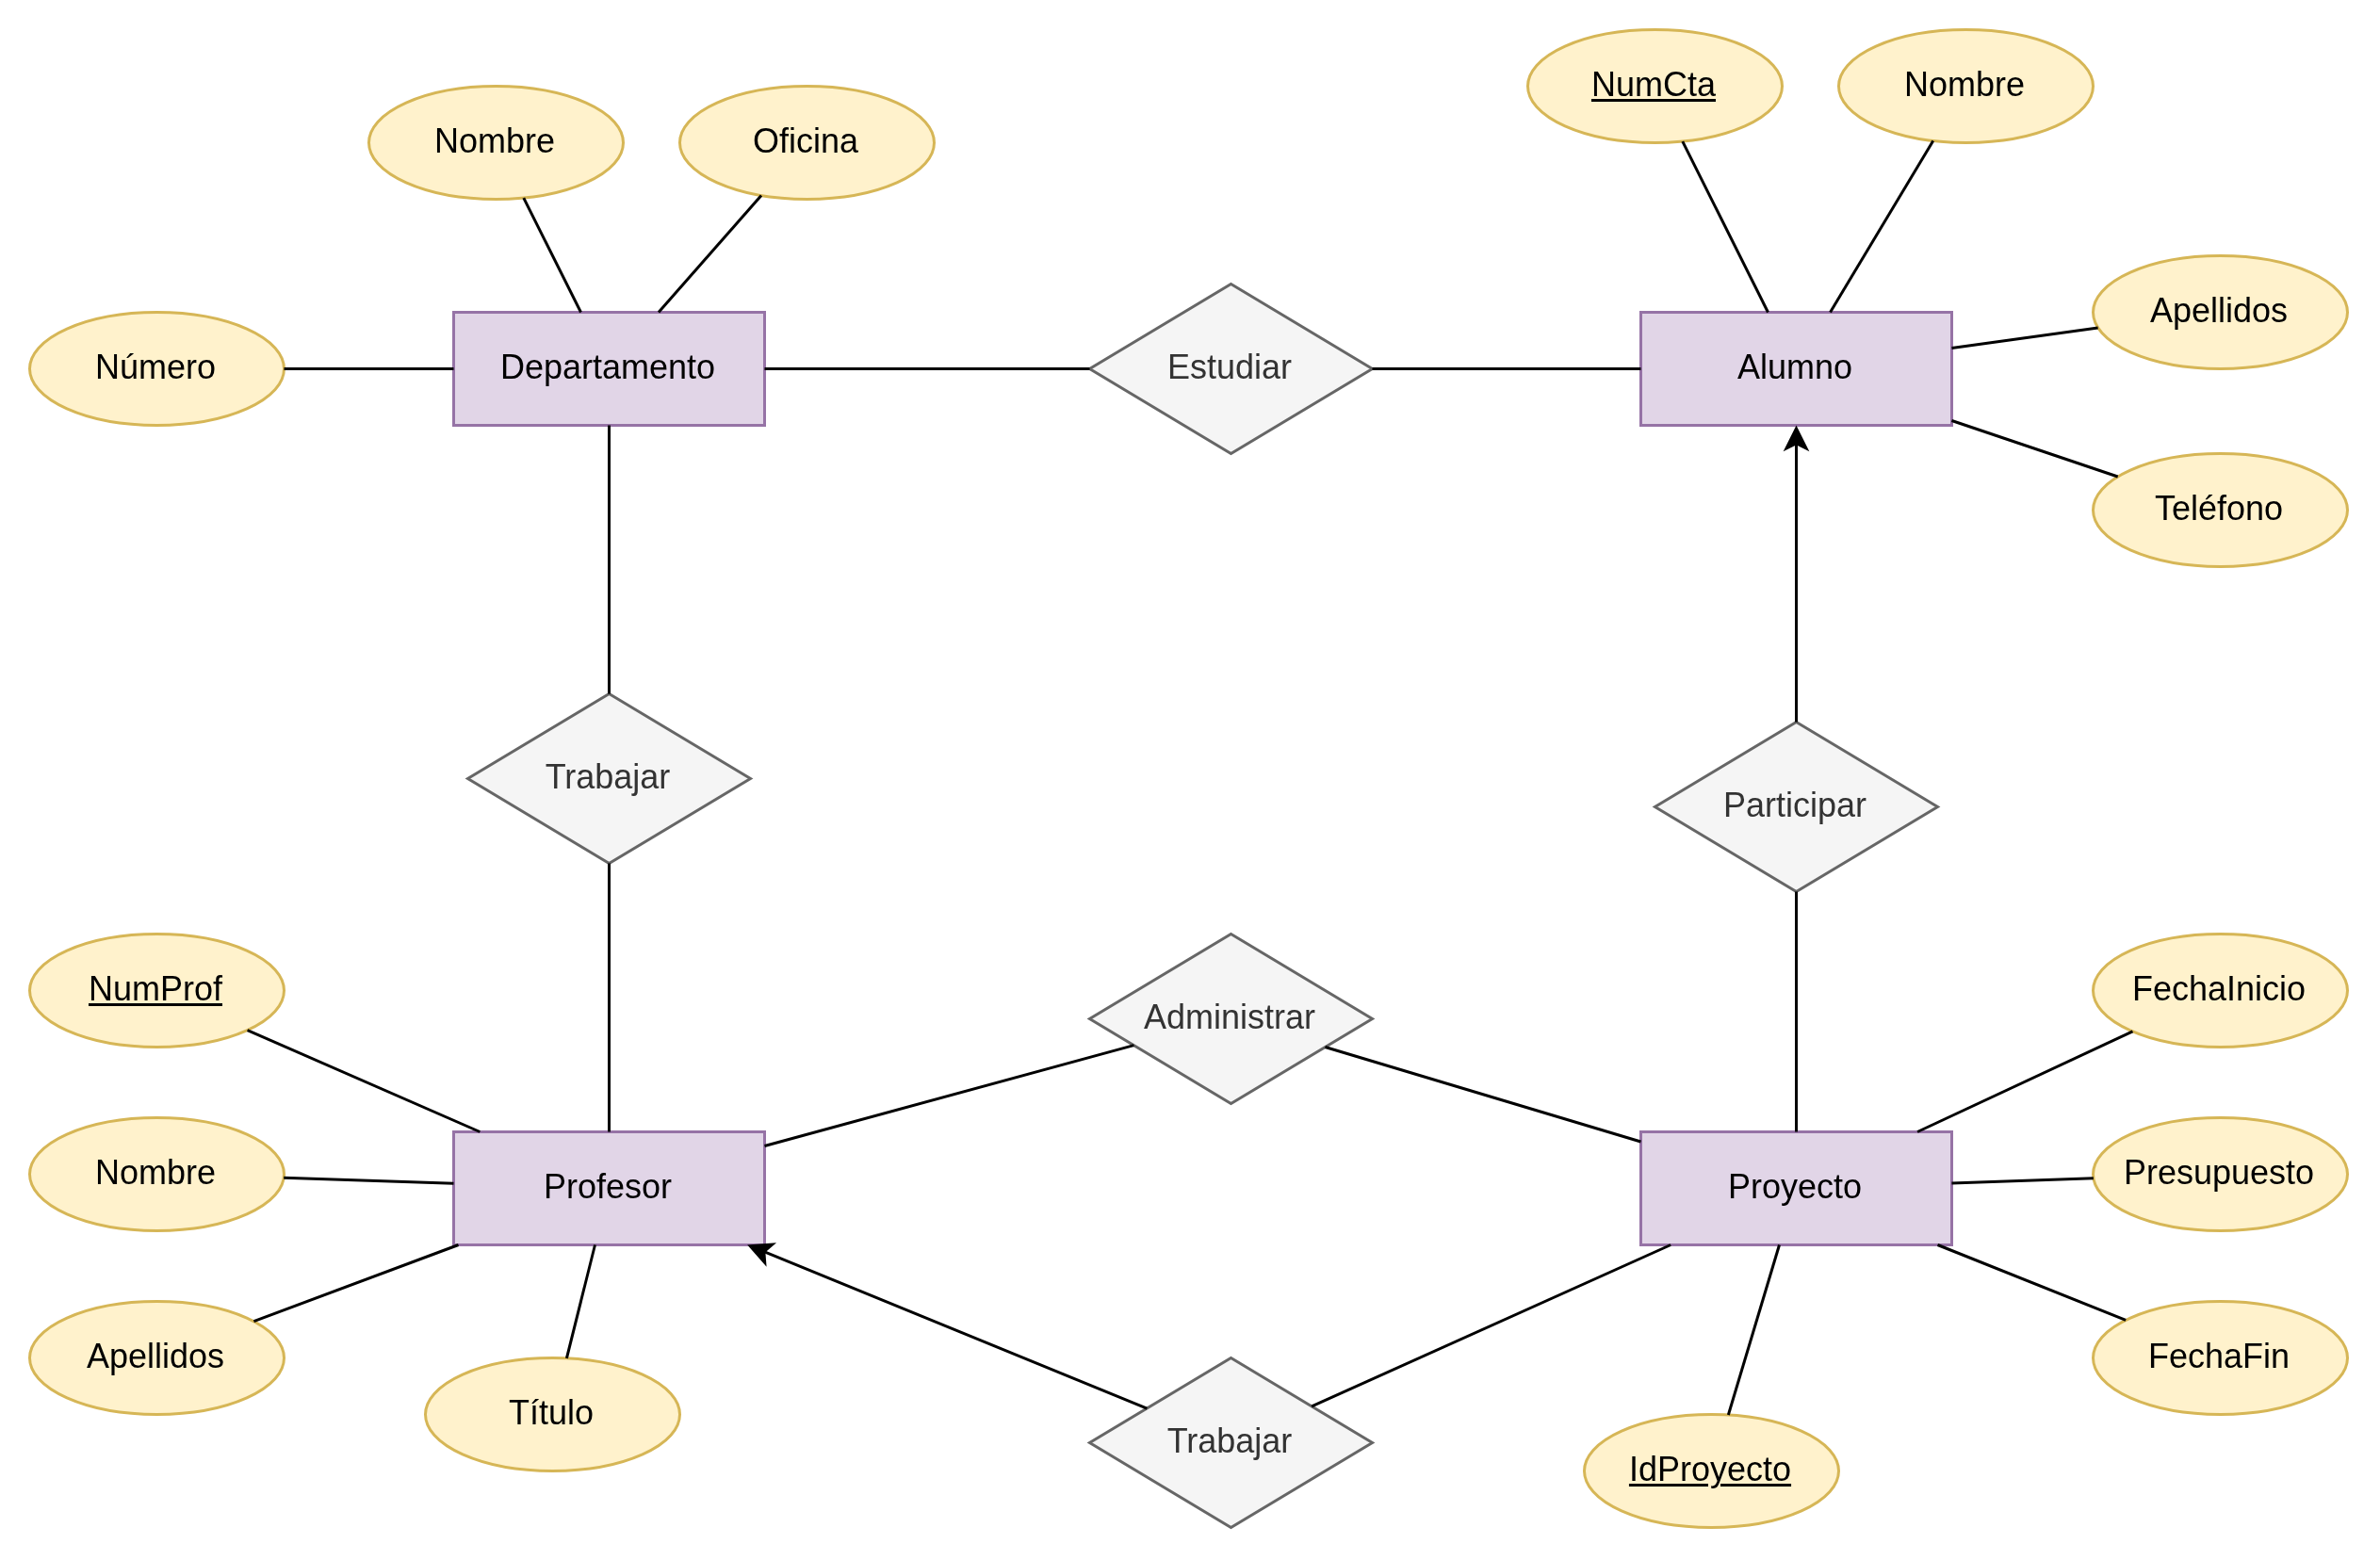
\includegraphics[width=\textwidth]{Figuras/ejercicio2ii.png}
	\caption{Modelo E-R de la base de datos de una universidad.}
	\label{fig:2ii}
\end{figure}

\begin{itemize}
	\item Dado que \textbf{solo los alumnos graduados pueden participar en proyectos}, se desea distinguir entre \textbf{alumnos graduados} y \textbf{no graduados}. Además de la información almacenada para un alumno, para los \textbf{alumnos graduados} se desea almacenar el \textbf{título} que posee y para los \textbf{alumnos no graduados} su \textbf{número de expediente}.
	\item Un \textbf{alumno graduado} puede ser \textbf{tutor} de varios \textbf{alumnos no graduados} y cada \textbf{alumno no graduado} tendrá \textbf{solamente un tutor}.
	\item Se desea almacenar, para cada \textbf{profesor}, el nombre del \textbf{cargo} que ocupa en cada \textbf{departamento} (el cual es \textbf{único dentro del departamento}) y la \textbf{carga horaria} asociada. Un mismo \textbf{cargo} puede tener \textbf{diferente carga horaria} dependiendo del departamento y/o del profesor. Dentro de un \textbf{departamento} no pueden existir \textbf{profesores} con el \textbf{mismo cargo}. Un \textbf{profesor} podrá tener el \textbf{mismo cargo} en varios departamentos.
	\item Cuando un \textbf{alumno graduado participa} en un \textbf{proyecto} y un \textbf{profesor debe supervisar su trabajo} en ese proyecto. Cada \textbf{alumno graduado} podrá trabajar en \textbf{múltiples proyectos}, en los cuales podrá ser supervisado por \textbf{diferentes profesores}.
\end{itemize}

Obtén un nuevo modelo E-R modificando el modelo presentado, para incorporar los cambios deseados. Identifica las restricciones de \textbf{cardinalidad}, \textbf{participación} e \textbf{identidad} en el nuevo modelo propuesto.

\medskip
\textbf{Modelo propuesto.}

\begin{figure}[H]
	\centering
	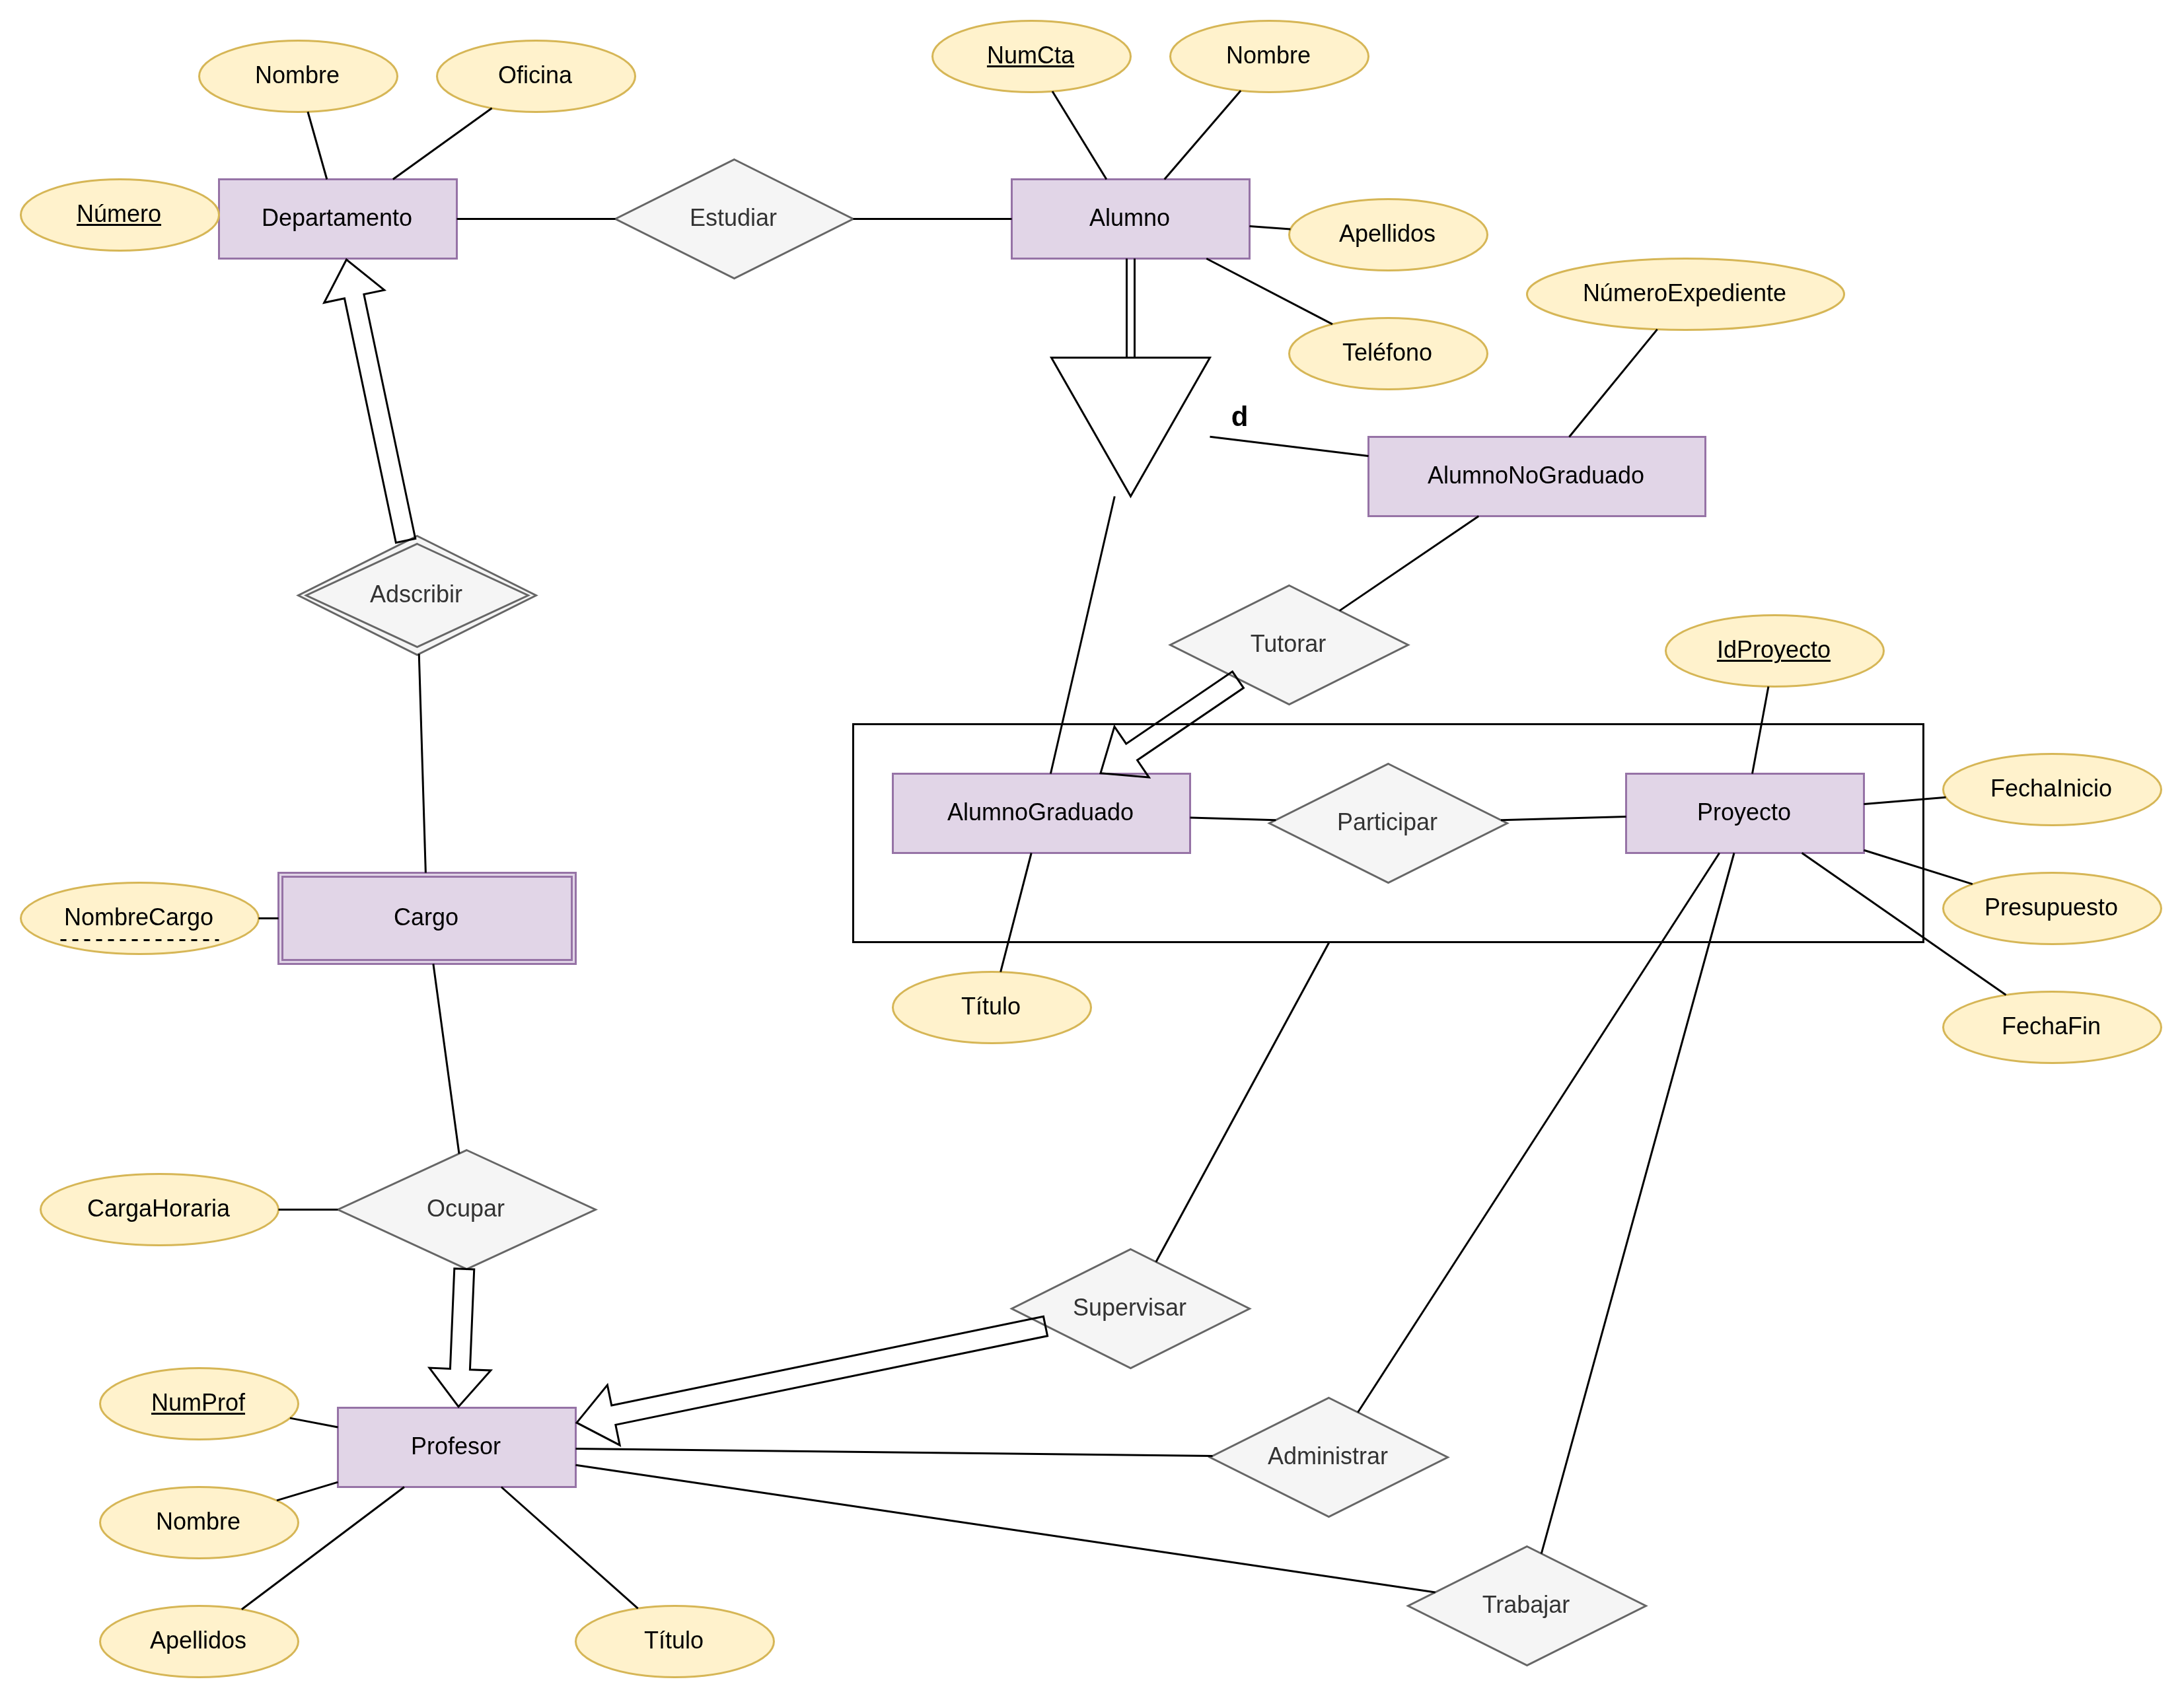
\includegraphics[width=\textwidth]{Figuras/2ii_universidad.png}
	\caption{Modelo E-R modificado de la base de datos de una universidad.}
	\label{fig:2ii-modelo}
\end{figure}

\textbf{Consideraciones de diseño:}

\textbf{1) Especialización de \textit{Alumno}.} Se modela una jerarquía sobre \textit{Alumno} con dos subclases, \textit{AlumnoGraduado} y \textit{AlumnoNoGraduado}. La especialización es \textbf{total} (todo alumno es graduado o no graduado) y \textbf{disjunta} (ningún alumno pertenece a las dos). Los atributos comunes (\textit{NumCta}, Nombre, Apellidos, Teléfono) permanecen en la superclase; se agrega \textit{Título} a los graduados y \textit{NúmeroExpediente} a los no graduados. Ambas subclases heredan \textit{NumCta} como identificador. Como sólo los graduados participan en proyectos, la relación con \textit{Proyecto} se conecta exclusivamente a \textit{AlumnoGraduado}.

\textbf{2) Tutoría.} Se agrega la relación binaria \textit{Tutorar} entre las dos subclases. Un alumno graduado puede tutelar a varios no graduados (1:N); cada no graduado tiene exactamente un tutor, por lo que del lado \textit{AlumnoNoGraduado} la participación es \textbf{total con cardinalidad 1}, y del lado \textit{AlumnoGraduado} es parcial.

\textbf{3) Cargo y carga horaria.} La restricción ``dentro de un departamento no puede haber dos profesores con el mismo cargo'' convierte al cargo en un dato identificable dentro del departamento; por ello se modela \textit{Cargo} como \textbf{entidad débil} de \textit{Departamento} con clave parcial \textit{NombreCargo}, de modo que su identificador es \textbf{(Número, NombreCargo)} y la unicidad queda garantizada por la estructura del modelo. La asignación profesor--cargo se representa con la relación \textit{Ocupar} (1:N): cada cargo lo ocupa exactamente un profesor (\textbf{total, 1}) y un profesor puede ocupar varios cargos (parcial, N), pudiendo repetir el mismo nombre de cargo en departamentos distintos. Como la \textbf{carga horaria} puede variar según el departamento y/o el profesor, se modela como \textbf{atributo de \textit{Ocupar}} y no de \textit{Cargo} ni de \textit{Profesor}.

\textbf{4) Supervisión en proyectos.} La supervisión recae sobre una \textit{participación} concreta (alumno, proyecto) y no sobre el alumno o el proyecto por separado; por eso se usa \textbf{agregación}: la relación \textit{Participar} (\textit{AlumnoGraduado}--\textit{Proyecto}) se trata como una unidad y se relaciona con \textit{Profesor} mediante \textit{Supervisar}. Cada participación tiene exactamente un profesor supervisor (\textbf{total, 1}) y un profesor puede supervisar varias participaciones (parcial, N), de modo que un alumno puede trabajar en varios proyectos supervisado por profesores distintos.

\textbf{5) Sin cambios.} Las relaciones \textit{Estudiar}, \textit{Administrar} y \textit{Trabajar} (Profesor--Proyecto) se conservan tal como estaban.

\textbf{Restricciones del modelo:}
\begin{itemize}
	\item \textbf{Cardinalidad:} \textit{Ocupar} y \textit{Tutorar} son 1:N; \textit{Supervisar} es N:1; \textit{Trabajar} (Profesor--Proyecto), \textit{Administrar} y \textit{Participar} son M:N.
	\item \textbf{Participación:} \textit{Cargo} participa \textbf{totalmente} en \textit{Adscribir} y en \textit{Ocupar}; \textit{AlumnoNoGraduado} participa \textbf{totalmente} en \textit{Tutorar}; la participación agregada de \textit{Participar} es \textbf{total} en \textit{Supervisar}. El resto de las participaciones son parciales.
	\item \textbf{Identidad:} \textit{Número} (Departamento), \textit{NumCta} (Alumno y sus subclases), \textit{NumProf} (Profesor) e \textit{IdProyecto} (Proyecto); la entidad débil \textit{Cargo} se identifica por \textbf{(Número, NombreCargo)}.
\end{itemize}
